% latexmk -pvc -pdf
\documentclass[12pt, a4paper, openany]{book}
\usepackage[margin=2.5cm]{geometry}
\usepackage{titling}
\usepackage{titlesec}
\usepackage{amsmath,amsthm,amsfonts,amssymb}
\usepackage{dsfont}
\usepackage{mathtools}
\usepackage{braket}
\usepackage[font=scriptsize,labelfont=bf]{caption}
\usepackage[english]{babel}
\usepackage{pdflscape} 
\usepackage{cite}

\usepackage{datetime}
\newdateformat{monthyeardate}{%
  \monthname[\THEMONTH], \THEYEAR}

\usepackage{graphicx}
\newenvironment{Figure}
    {\par\medskip\noindent\minipage{\linewidth}}
    {\endminipage\par\medskip}
\usepackage{tabularx}

\newenvironment{abstract}
{\clearpage \thispagestyle{empty} \null \vfill \begin{center} \bfseries \large Abstract \end{center}}
{\vfill \null \clearpage}

% Colours:
\usepackage[table]{xcolor} % for setting colors
\definecolor{purple}{RGB}{117,77,226}

\usepackage[bookmarksopen,
  pagebackref,
  pdfpagelayout=TwoPageRight,
  colorlinks=true,
  urlcolor=purple,
  citecolor=purple,
  filecolor=purple,
  linkcolor=purple,
  ]
{hyperref}

\usepackage{listings}
\usepackage{xcolor} % Necessary to define custom colors

\definecolor{softblue}{rgb}{0.3, 0.5, 0.8}
\definecolor{darkergreen}{rgb}{0, 0.5, 0}

\lstset{
  basicstyle=\ttfamily\small, % Set the typeface to typewriter and small size
  breaklines=true, % Enable line breaking
  postbreak=\mbox{\textcolor{red}{$\hookrightarrow$}\space}, % Marker for line breaks
  numbers=left, % Line numbers on left
  numberstyle=\tiny, % Set the size of the numbers
}

\lstdefinestyle{mystyleC}{
    language=C,      
    commentstyle=\color{softblue},
    morecomment=[l]{//},  % Line comment
}

\lstdefinestyle{mystylePython}{
    language=Python,      
    commentstyle=\color{darkergreen},
    morecomment=[l]{//},  % Line comment
}

\titleformat{\chapter}[display]
  {\normalfont\bfseries}{}{0pt}{\Huge}


% Required packages
\usepackage{catchfile}

% Command to execute texcount and capture the word count
\newcommand\wordcount[1]{
    \immediate\write18{texcount #1.tex | grep "Words in text" | cut -d: -f2 > #1.wordcount.tmp}
    \CatchFileDef{\mywordcount}{#1.wordcount.tmp}{}
    \immediate\write18{rm #1.wordcount.tmp} % to remove the temporary file
    \mywordcount % to print the word count
}

\begin{document}

\begin{titlepage}
\begin{center}
    {\Huge BEDSAT:Antarctica}\\ [1cm] 
    % {\Large random writings}\\ [2cm]
    % {\Large random writings}\\ [2cm]
    \vspace{3cm}
    {\large Ana Fabela Hinojosa\footnote{ana.fabelahinojosa1@monash.edu}}\\ [1cm]
    Supervisors:\\
    Dr. Felicity McCormack\\
    Dr Jason Roberts\\
    Dr Richard Jones\\ [2cm]
    \monthyeardate\today\\ [9.5cm]
    \end{center}
    
\includegraphics[scale=0.12]{monash.jpg}
\includegraphics[scale=0.6]{SAEF.png}\\ [1cm]

\end{titlepage}


%----------------------------------------------------------------------------------------
%   QUOTATION PAGE
%----------------------------------------------------------------------------------------
% \vspace*{0.2\textheight}

% \noindent{``El alacrán clavándose el aguijón, harto de ser un alacrán pero necesitando de su alacranidad para acabar con el alacrán''.}\bigbreak
% % \vspace{-2cm}
% \hfill Julio Cortázar\bigbreak

\begin{abstract}\label{abstracc}
Antarctica has been losing ice mass over recent decades, contributing to rising sea levels (SLR). There is significant uncertainty regarding the extent and timing of this ice loss. One key factor influencing ice flow and loss is bed topography, typically derived from sparse airborne radar surveys. The uncertainty in the data can impact simulations of the Antarctic Ice Sheet (AIS) evolution under climate change.
We need alternative approaches to surveying Antarctica and given the logistical challenges we plan on modelling the bed topography.
Our model's accuracy (surely?) depends on the spacing of ice thickness measurements and uncertainties in ice velocity (SOMETHING I AM WORKING ON understanding rn) and surface mass balance. 
BedSAT, aims to leverage the mathematical relationship between ice surface elevation (data we have?) and bed topography to estimate the actual bed topography of a surrounding spatial region (in 2D?). 
\end{abstract}


% \chapter*{Acknowledgements}

% \tableofcontents
% \chapter{An example of previous work modelling the bedrock topography}\label{n1}

Numerical modelling, sedimentary sequence interpretation suggest cyclical periods of ice-sheet expansion and retreat\cite{Young2011}. Using ice-penetrating radar data to generate a new basal bed topography of the Aurora Subglacial Basin (ASB) in east Antarctica is characterised by a fjord landscape (this land is under $\sim$ under $2-4.5$ km of ice). The ASB has a potentially significant influence on the east Antarctic ice-sheet (EAIS), however there is high uncertainty in estimates of past and present global sea level changes due to the scarcity of bed data\cite{Young2011}. This uncertainty also limits the accuracy of models used to predict future ice sheet growth or decay.\\

{\large Methods in\cite{Young2011}}
\begin{enumerate}
    \item A ski-equipped airplane (DC-3T) carried a radar system (HiCARS), which can see through ice. HiCARS sends signals that bounce back to show the thickness of the ice and the shape of the land beneath it.
    \item The plane flew back and forth over a large area, covering distances of around 1,000 km. The flights took place over two different periods in 2008–2009 and 2009–2010.
    \item The radar data was cleaned up (processed) to improve accuracy, and they used a special radar system that helps reduce distortions (errors) in the measurements. \textbf{[HOW?]}
    \item Thickness of the ice was measured using the time it took for the radar signals to travel through the ice and back, assuming the radar signals move through the ice at a specific speed (169 meters per microsecond).
    \item The height of the land below the ice was calculated by looking at the radar-determined surface of the ice. \textbf{[WHAT?]}
    \item The radar data was combined with other existing datasets (BEDMAP) to improve the overall picture. They used a computer algorithm to fill in gaps where they didn’t have direct measurements. \textbf{[WHICH?]}
    \item Determining how rough or uneven the land under the ice was, by using a statistical measure called the ''root mean squared (rms) deviation."
\end{enumerate}

In short, Young et al. used advanced radar technology on an airplane to map the ice thickness and the landscape beneath it in a region of Antarctica, combining this data with previous maps for a better overall picture.

\chapter{IPCC Special Report 2019}\label{n2}
\textbf{WHY IS IMPORTANT TO DEVELOP BETTER TOPOGRAPHIC MODELS OF THE ANTARCTIC CONTINENT?}
The polar regions are losing ice, and their oceans are changing rapidly. The consequences of this polar transition extend to the whole planet and it is crucial for us to understand them and plan for changes.
\begin{itemize}
\item Climate-induced changes in seasonal ice extent and thickness are affecting sea ice and ocean layers, which impacts marine plant growth (highly likely). This alters ecosystems (moderately likely). The timing and amount of plant growth have changed in both polar oceans, varying by location (highly likely). In Antarctica, these changes relate to retreating glaciers and sea ice change (moderately likely). In the Arctic, they've affected the types, locations, and numbers of marine species, changing ecosystem structure (moderately likely)\cite{O_C_in_changingClimate}.
\item The rapid ice loss from the Greenland and Antarctic ice sheets during the early 21st century has increased into the near present day, adding to the ice sheet contribution to global sea level rise (extremely likely)\cite{O_C_in_changingClimate}.
\item Both polar oceans will be increasingly affected by $\mathrm{CO_2}$ uptake, causing conditions corrosive for calcium carbonate shell-producing organisms (high confidence), with associated impacts on marine organisms and ecosystems (medium confidence)\cite{O_C_in_changingClimate}.
\item change in thermohaline circulation....
\end{itemize}

Temperature changes in Antarctica:
Unlike the Arctic, which has seen uniform warming, Antarctica's temperature changes have been less consistent. West Antarctica has warmed in some parts. East Antarctica hasn't shown significant overall change. in the past 3-5 decades. There's low confidence in these observations due to limited data and high variability.

Why Antarctica isn't warming as much as the Arctic:
The Southern Ocean surrounding Antarctica absorbs and mixes heat deep into the ocean\cite{L_T_C_C}.


Factors influencing Antarctic climate:

Three main atmospheric patterns affect Antarctica's climate and sea ice:
a) Southern Annular Mode (SAM)
b) Pacific South American mode
c) Zonal-wave 3


Recent changes in the Southern Annular Mode (SAM):

The SAM has been mostly positive in recent decades during summer.
This means stronger westerly winds around Antarctica.
This positive phase is unprecedented in at least 600 years.
It's associated with cooler conditions over Antarctica.


Causes of SAM changes:

Ozone depletion was likely the main driver of SAM changes from the late 1970s to late 1990s.
Since 2000, tropical sea surface temperatures have played a stronger role in influencing SAM.


Other influences on Antarctic climate:

Tropical sea surface temperatures can affect Antarctic temperatures and Southern Hemisphere mid-latitude circulation\cite{JACOBS_2004}.



In summary, Antarctica's climate is complex and influenced by various factors, with recent changes differing from those in the Arctic due to unique ocean and atmospheric patterns.

\begin{Figure}
\centering
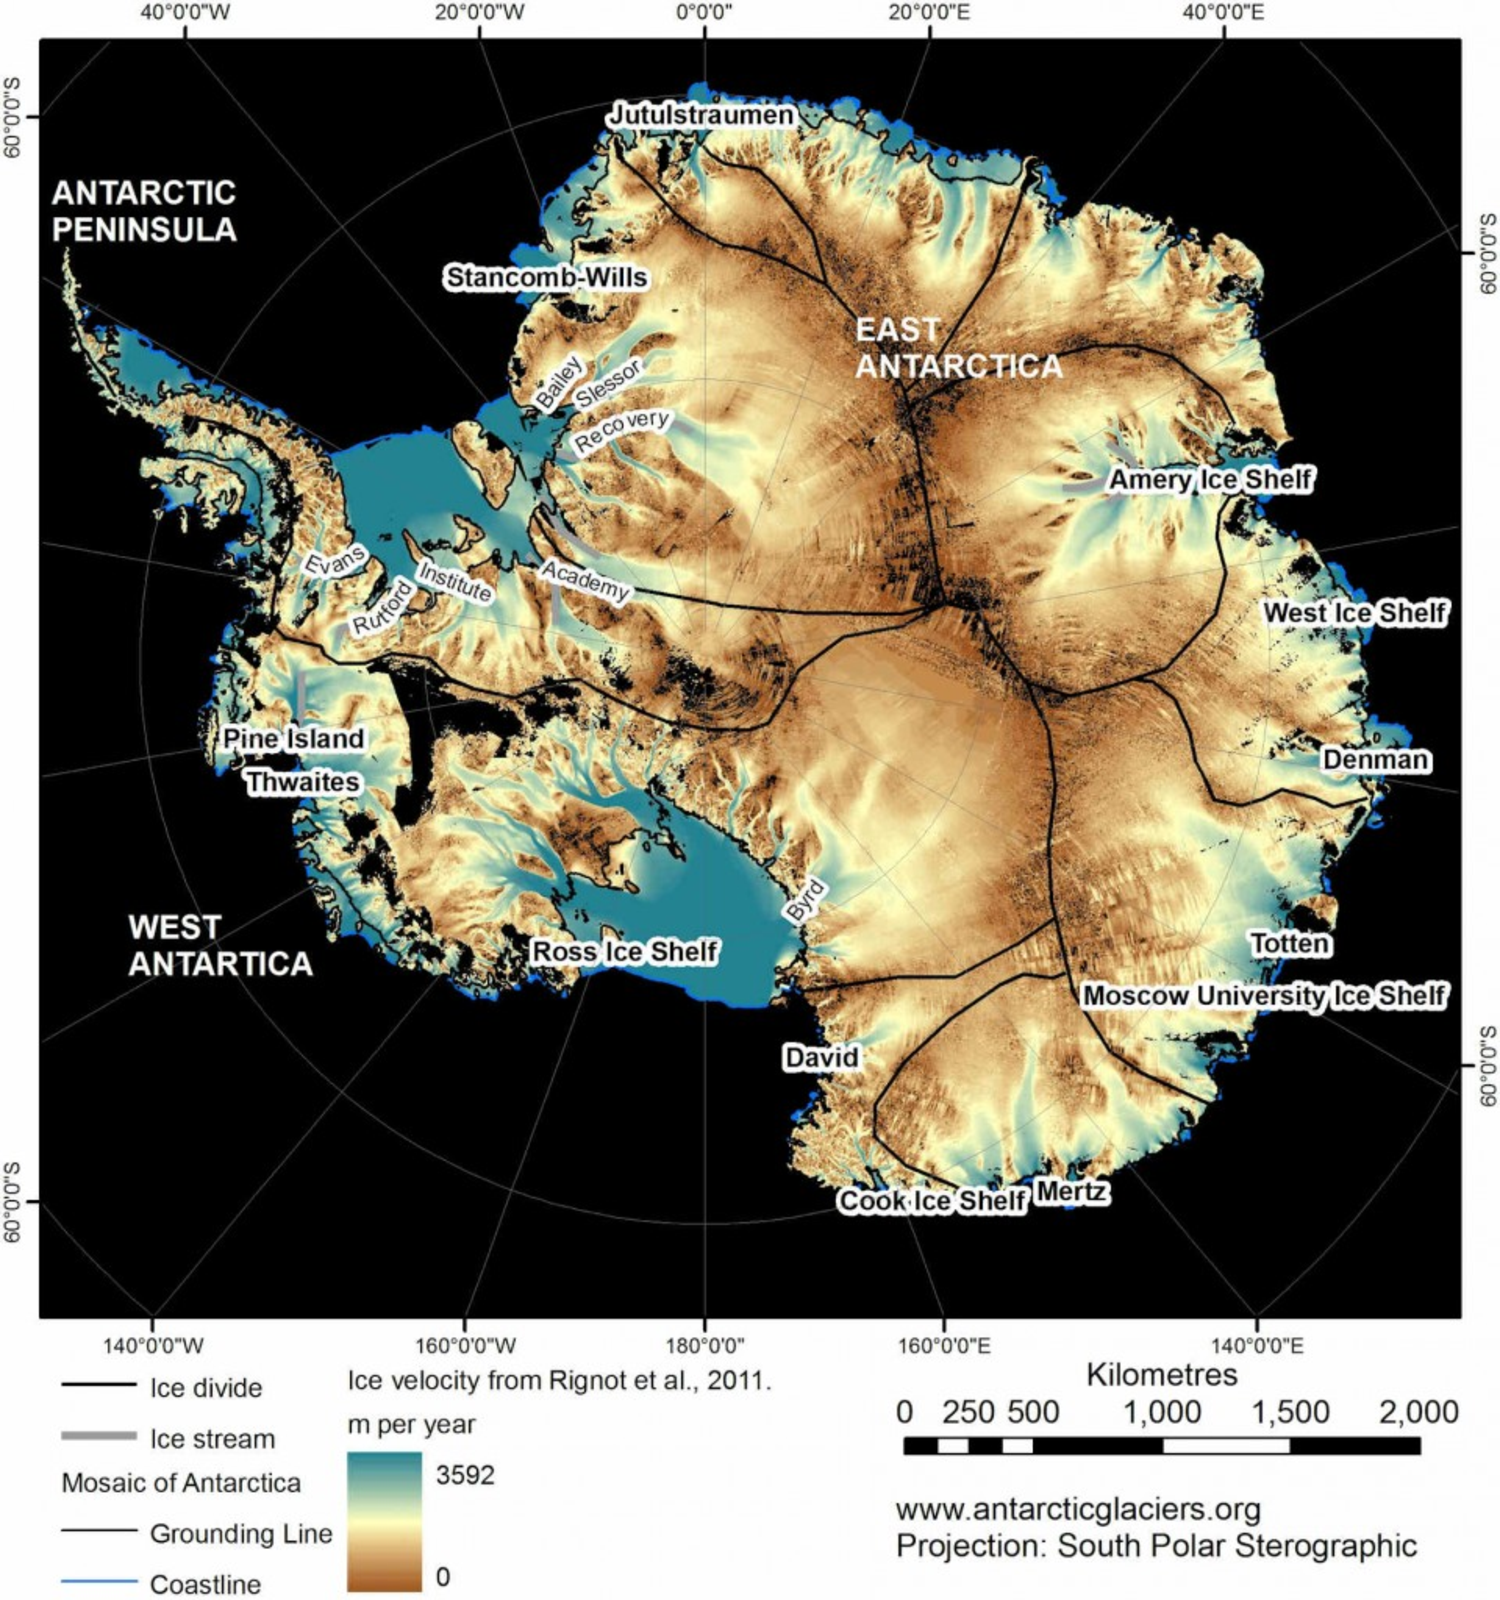
\includegraphics[width=1.1\linewidth]{antarctica_velocity.pdf}
\captionof{figure}{}
\label{fig:Antarctica_velocity}
\end{Figure}

Unknown terms
{\small \begin{itemize}
\item{Channel incision}
\item{Alpine style glaciation}
\end{itemize}
}
\vspace{1cm}
TOOLS
{\small \begin{itemize}
\item{ICECAP aero geophysical programme}
\item{BEDMAP}
\end{itemize}
}
\vspace{1cm}
MATHS
{\small \begin{itemize}
\item{Lagrangian interpolation}
\item{natural-neighbour interpolation}
\end{itemize}
}


% \wordcount{notes1} words in this section.

\chapter{Why Understanding Antarctica's Landscape Matters: Climate Impacts and Global Significance}\label{n1}

The polar regions are losing ice, and their oceans are changing rapidly\cite{O_C_in_changingClimate}. The consequences of this polar transition extend to the whole planet and it is crucial for us to understand them and plan for changes.
\begin{itemize}
\item Climate-induced changes in seasonal ice extent and thickness are affecting sea ice and ocean layers, which impacts marine plant growth (highly likely). This alters ecosystems (moderately likely). The timing and amount of plant growth have changed in both polar oceans, varying by location (highly likely). In Antarctica, these changes relate to retreating glaciers and sea ice change (moderately likely). In the Arctic, they've affected the types, locations, and numbers of marine species, changing ecosystem structure (moderately likely)\cite{O_C_in_changingClimate}.
\item The rapid ice loss from the Greenland and Antarctic ice sheets during the early 21st century has increased into the near present day, adding to the ice sheet contribution to global sea level rise (SLR)(extremely likely)\cite{O_C_in_changingClimate}.
\item Both polar oceans will be increasingly affected by $\mathrm{CO_2}$ uptake, causing conditions corrosive for calcium carbonate shell-producing organisms (high confidence), with associated impacts on marine organisms and ecosystems (medium confidence)\cite{O_C_in_changingClimate}.
\item Thermohaline circulation changes: a large-scale system of ocean currents driven by differences in water temperature (thermo) and salinity (haline), these factors affect the density of seawater. Thermohaline circulation plays a critical role in regulating Earth's climate and distributing heat and nutrients across the globe. Warm surface waters flow from the tropics toward the poles, where they cool and sink, forming deep-water currents. These deep waters then travel along the ocean floor toward the equator, eventually rising to the surface through a process called upwelling, bringing cold, nutrient-rich waters to the surface\cite{JACOBS_2004}. Altering the salt concentration in the Antarctic ocean due to the melting of the ice sheet could result in disruptions to this circulation and could have significant consequences for global weather systems.
\end{itemize}

Unlike the Arctic, which has seen uniform warming, Antarctica's temperature changes have been less consistent. West Antarctica has warmed in some parts. East Antarctica hasn't shown significant overall change. in the past 3-5 decades. There's low confidence in these observations due to limited data and high variability\cite{O_C_in_changingClimate}. \\\\
\textbf{Atmospheric factors influencing Antarctic climate:}
\begin{itemize}
\item Southern Annular Mode (SAM)\\
    \textbf{Recent changes in the Southern Annular Mode (SAM):} The SAM has been mostly positive in recent decades during summer. This means stronger westerly winds around Antarctica. This positive phase is unprecedented in at least 600 years. It's associated with cooler conditions over Antarctica\cite{O_C_in_changingClimate}.\\
    \textbf{Causes of SAM changes:} Ozone depletion was likely the main driver of SAM changes from the late 1970s to late 1990s. Since 2000, tropical sea surface temperatures have played a stronger role in influencing SAM\cite{O_C_in_changingClimate}.\\
    \textbf{Other influences on Antarctic climate:} Tropical sea surface temperatures can affect Antarctic temperatures and Southern Hemisphere mid-latitude circulation\cite{JACOBS_2004}.
\item Pacific South American mode
\item Zonal-wave 3
\end{itemize}

\textbf{Other factors influencing Antarctic climate:}
\begin{itemize}
\item Antarctica isn't warming as much as the Arctic because the Southern Ocean surrounding Antarctica absorbs and mixes heat deep into the ocean\cite{L_T_C_C}.
\end{itemize}
\wordcount{why_it_matters} words in this section.

\chapter{Topographic Models of Antarctica: A Review}\label{n2}
Numerical modelling and sedimentary sequence interpretation suggest cyclical periods of ice-sheet expansion and retreat\cite{Young_2011}. Using ice-penetrating radar data to generate a new basal bed topography of the Aurora Subglacial Basin (ASB) in east Antarctica is characterised by a fjord landscape (this land is under $\sim$ under $2-4.5$ km of ice). The ASB has a potentially significant influence on the east Antarctic ice-sheet (EAIS), however there is high uncertainty in estimates of past and present global sea level changes due to the scarcity of bed data\cite{Young_2011}. This uncertainty also limits the accuracy of models used to predict future ice sheet growth or decay.\\
{\large Methods in\cite{Young_2011}}
\begin{enumerate}
    \item A ski-equipped airplane (DC-3T) carried a radar system (HiCARS), which can see through ice. HiCARS sends signals that bounce back to show the thickness of the ice and the shape of the land beneath it.
    \item The plane flew back and forth over a large area, covering distances of around 1,000 km. The flights took place over two different periods in 2008–2009 and 2009–2010.
    \item The radar data was cleaned up (processed) to improve accuracy, and they used a special radar system that helps reduce distortions (errors) in the measurements. \textbf{[HOW?]}
    \item Thickness of the ice was measured using the time it took for the radar signals to travel through the ice and back, assuming the radar signals move through the ice at a specific speed (169 meters per microsecond).
    \item The height of the land below the ice was calculated by looking at the radar-determined surface of the ice. \textbf{[WHAT?]}
    \item The radar data was combined with other existing datasets (BEDMAP) to improve the overall picture. They used a computer algorithm to fill in gaps where they didn’t have direct measurements. \textbf{[WHICH?]}
    \item Determining how rough or uneven the land under the ice was, by using a statistical measure called the ''root mean squared (rms) deviation."
\end{enumerate}
In short, Young et al. used advanced radar technology on an airplane to map the ice thickness and the landscape beneath it in a region of Antarctica, combining this data with previous maps for a better overall picture.

\wordcount{a_review} words in this section.

\chapter{Ice is weird}
Ice is described as non-Newtonian because its viscosity $(\nu)$ is not constant. A Newtonian fluid (like water) has a constant viscosity regardless of the flow conditions, while a non-Newtonian fluid's viscosity changes based on factors like strain rate. The viscosity of ice depends on how much it’s deforming (shear rate).
Ice is a slow, shear-thinning fluid. "shear-thinning" means that the viscosity of ice decreases with increasing strain rate. This means that under more strain forces ice becomes "softer" and flows more easily."Slow" means that the flow of ice occurs at very low velocities, that means that the change in flow velocity (time dependent and convective) are approximately zero
\begin{equation}
\rho(\vec{u_t} + \vec{u} \dotp \nabla \vec{u}) \approx 0,
\end{equation}
This assumptiongreatly simplifies the Navier-Stokes equations for ice flow.
The equations we use to are the incompressibility condition (the divergence of the velocity field is zero)
\begin{equation}
\nabla \vec{u}) = 0,
\end{equation}
the force balance equation, i.e. the pressure gradient, the divergence of the stress tensor (viscous forces within the ice) and the gravitational body force acting on the ice all cancel out
\begin{equation}
-\nabla p + \nabla\dot\tau_{ij} + \rho g,
\end{equation}
And finally Glen flow law
\begin{equation}
D_{ij} = A\tau^{n} \tau_{ij},
\end{equation}
where the strain rate tensor $D_{ij}$, which describes how fast the ice is deforming is proportional to the deviatoric stress tensor $\tau_{ij}$ and it's magnitude $\tau$, which accounts for the stress caused by deformation (as opposed to isotropic stress like pressure). is the flow law exponent, which determines how strongly the flow rate depends on stress. For ice, Glen's law uses $n=3$, which implies a nonlinear relationship between stress and strain rate, meaning the flow rate accelerates rapidly with increased stress\cite{modelling_ppt}.

This model does not have time derivatives!?

\section{Ice flow over bedrock perturbations}
This 1970's rheology paper by Budd explains how bedrock irregularities beneath a glacier affect the surface shape of the ice mass. Budd develops a mathematical model to describe the flow of ice over these undulations, considering the ice as a viscous fluid that deforms under stress. The model predicts that the surface shape of the glacier will mirror the bedrock undulations, but shifted out of phase by approximately $\frac{\pi}{2}$ radians. The paper analyzes the damping of different wavelengths of bedrock undulations, finding that waves with a length roughly three times the ice thickness are minimally damped, while shorter or longer waves are significantly damped out. Finally, the implications of this theory proposes the potential for ice to flow uphill, concluding that bedrock undulations with wavelengths several times the ice thickness are most important in controlling ice motion.

% \section{Temperate Ice Sliding: An Empirical Study}
% % Static and dynamic friction are different.
% % Limiting static shear stress: is the tipping point where pressure overcomes friction and sliding begins. The interface of ice on bedrock has very high static friction.

% % how does the ice respond to different surfaces (smooth, rough, different material compositions)?
% % how does the sliding speed varies from one surface to another?
% % Rough surfaces requires more force to overcome static friction.

% % Glaciers carve away landscapes via friction and the landscape makes the ice slide.

% The main objectives described in\cite{Budd_Keage_Blundy_1979} are to describe the relationship between forces and ice movement (sliding) over different surfaces, and how the moving ice affects the surfaces over which they slide.

% \begin{enumerate}
% \item How did the researchers apply normal and shear stresses to the ice blocks in their experiments?

% \item Describe the relationship between limiting static shear stress and normal load observed in the experiments.

% \item How did sliding velocity vary with shear stress and normal stress at low normal loads? % The experiments showed a direct proportionality between limiting static shear stress and normal load, indicating a constant coefficient of limiting friction specific to each slab.

% \item What was the significance of the product (TmVb) in the experiments?
% % The product TmVb, representing the transition point from steady-state sliding to acceleration, tended towards a constant value, suggesting a critical threshold for dynamic instability.

% \item How did the relationship between sliding velocity and shear stress change at high normal loads?
% % At low normal loads, sliding velocity increased proportionally with shear stress and decreased proportionally with both normal load and surface roughness.
% % "The sliding speed at high stresses is not linear, velocity increases with the cube of the shear stress*???* small force increase can lead to a lot of speed!
% % At high normal loads, the relationship shifted from linear to cubic, with sliding velocity increasing proportionally to the cube of shear stress and inversely proportionally to normal stress.


% \item What effect does an increase in the water table have on the effective normal stress acting on the glacier base?
% % An increase in the water table elevates the basal water pressure, which counteracts the normal stress from the overlying ice, effectively reducing the effective normal stress acting on the glacier base.

% \item Explain how the study's findings might help explain the high velocities observed in fast-outlet polar glaciers.
% % The study demonstrated that sliding velocity is highly sensitive to effective normal stress. For fast-outlet polar glaciers, where the base is often below sea level, the buoyancy effect of seawater can significantly reduce the effective normal stress, potentially leading to higher sliding velocities.

% \item What was the observed relationship between erosion and the experimental parameters (normal stress, shear stress, and velocity)?
% % Erosion was found to increase with higher normal stress, shear stress, and velocity, suggesting a combined effect of these parameters on the rate of material removal from the slab surface.

% \item Why did the researchers conclude that ice deformation, rather than regelation, plays a dominant role in the observed sliding behaviour?
% \end{enumerate}% The observed cubic relationship between sliding velocity and shear stress at high normal loads pointed towards ice deformation, rather than regelation, as the dominant mechanism governing sliding behaviour at the experimental scales.
    

% Essay Questions
% \begin{enumerate}
% \item Discuss the limitations of the experimental setup used in the study and how these limitations might affect the applicability of the findings to real-world glacier systems.
% \item Compare and contrast the roles of regelation and ice deformation in glacier sliding, drawing upon the findings of the study to support your arguments.
% \item Analyze how the study's results contribute to a better understanding of the dynamics of glacier surges, focusing on the factors that lead to the onset and propagation of surge events.
% \item Explain the concept of effective normal stress in the context of glacier sliding and discuss how variations in basal water pressure can influence glacier flow.
% \item Critically evaluate the significance of the study's findings for modelling glacier behaviour and predicting future glacier response to climate change.
% \end{enumerate}
    
    

\wordcount{icy_stuff} words in this section.

\chapter{Numerics}
\begin{Figure}
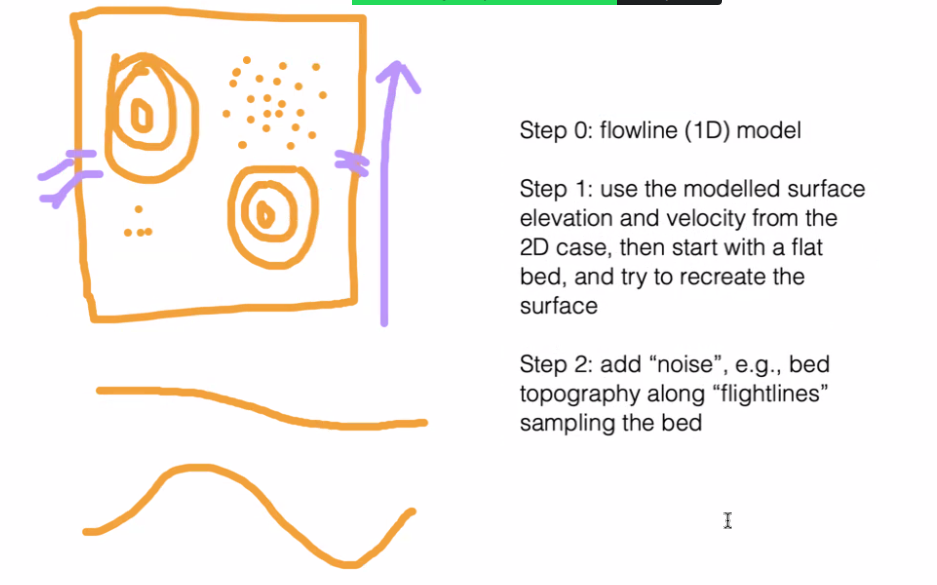
\includegraphics[width=0.9\linewidth]{steps.png}
\captionof{figure}{TODO}
\label{fig:first_sims}
\end{Figure}

\begin{Figure}
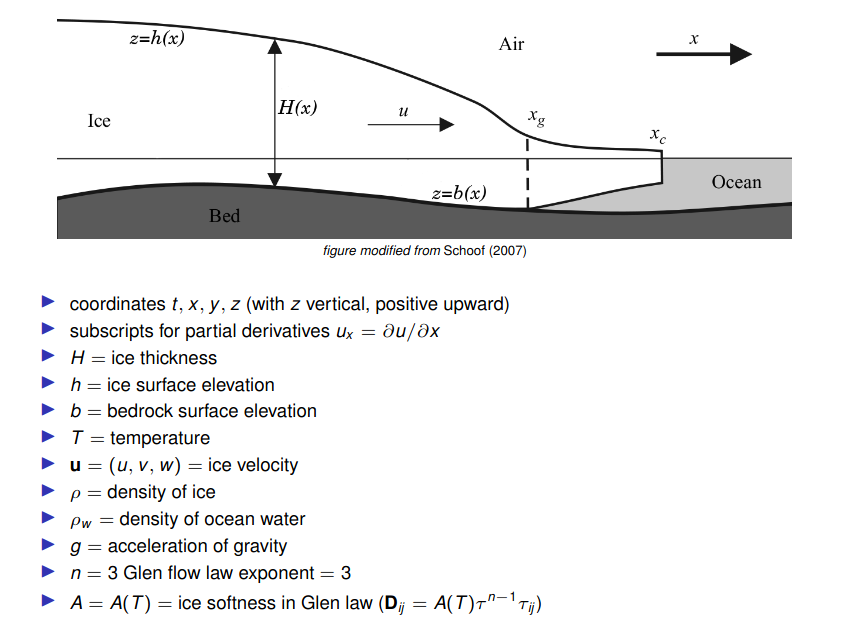
\includegraphics[width=0.9\linewidth]{numerical_modelling_of_glaciers.png}
\captionof{figure}{figure taken from\cite{modelling_ppt}}
\label{fig:parameters}
\end{Figure}

\section{ISSM: Continental-Scale Ice Sheet Modelling}
The Ice Sheet System Model (ISSM) was developed and is used for simulating ice sheet flow at continental scales. ISSM, a finite element, thermomechanical model, incorporates high-order stresses and high spatial resolution capabilities\cite{ISSM}. The Larour et al. (2012) ISSM paper discusses the different ice flow models within the software, including the full-Stokes, Blatter-Pattyn, Shallow-Shelf, and Shallow Ice Approximations, highlighting their individual strengths and limitations. It also explores numerical methods employed, such as static adaptive mesh refinement and inverse methods for parameter estimation. Finally, the study showcases the application of ISSM to the Greenland Ice Sheet, demonstrating its capacity to model the ice flow velocity with high accuracy, using data assimilation techniques to infer the basal drag coefficient.


% Study Guide
% Glossary of Key Terms

%     Shallow Ice Approximation (SIA): A simplified ice flow model that considers only vertical shear stresses and neglects horizontal stress gradients. Suitable for slow-moving ice in the interior of ice sheets.
%     Shallow Shelf Approximation (SSA): A simplified ice flow model that neglects vertical shear stresses and assumes depth-independent horizontal velocity. Appropriate for modeling floating ice shelves and fast-flowing ice streams.
%     Blatter-Pattyn Approximation (BP): A higher-order ice flow model that incorporates longitudinal stresses, making it suitable for simulating fast-flowing ice streams and regions with significant vertical shear.
%     Full-Stokes (FS): The most comprehensive and computationally expensive ice flow model, accounting for all stress components. Essential for accurately simulating ice flow near grounding lines.
%     Ice Sheet System Model (ISSM): A finite element, thermomechanical ice flow model that incorporates SIA, SSA, BP, and FS formulations to simulate ice sheet behaviour at various complexities and spatial resolutions.
%     Finite Element Method (FEM): A numerical method for solving partial differential equations by dividing the domain into smaller elements and approximating the solution within each element.
%     Adaptive Mesh Refinement: A technique used to refine the mesh in regions of high variability or complexity, enhancing model accuracy and efficiency.
%     Data Assimilation: The process of incorporating observational data into a model to improve its accuracy and predictive capabilities.
%     Basal Drag Coefficient: A parameter representing the frictional resistance between the ice sheet base and the underlying bedrock.
%     Grounding Line: The boundary where the ice sheet transitions from grounded ice to floating ice (ice shelf).
%     Calving: The process by which icebergs break off from the edge of a glacier or ice sheet.
%     InSAR: Interferometric Synthetic Aperture Radar, a remote sensing technique used to measure ice surface velocity.

% Quiz

% Instructions: Answer the following questions in 2-3 sentences.

%     What are the limitations of the Shallow Ice Approximation (SIA) and Shallow Shelf Approximation (SSA) in ice sheet modelling?
%     Why is the Full-Stokes (FS) model considered the most accurate representation of ice flow, and what makes its application challenging?
%     How does the Ice Sheet System Model (ISSM) integrate different ice flow approximations?
%     What is the importance of anisotropic adaptive mesh refinement in ISSM?
%     Describe the role of data assimilation in improving the accuracy of ice sheet models.
%     Why is the basal drag coefficient a crucial parameter in ice flow modeling?
%     Explain the concept of grounding line dynamics and its significance.
%     What is the process of calving, and why is it relevant to ice sheet mass balance?
%     How does ISSM handle the thermal regime of ice sheets?
%     What are some key challenges and future directions in ice sheet modeling using ISSM?

% Quiz Answer Key

%     SIA neglects horizontal stress gradients and is unsuitable for fast flow, while SSA ignores vertical shear, limiting accuracy near grounding lines.
%     FS accounts for all stress components, making it highly accurate, but its computational expense poses a challenge for large-scale applications.
%     ISSM offers SIA, SSA, BP, and FS formulations, allowing for different levels of complexity and computational efficiency.
%     It concentrates elements in dynamic regions like fast-flowing outlets, optimizing computational resources while preserving accuracy.
%     Data assimilation incorporates observations (e.g., surface velocity) to constrain model parameters and improve realism.
%     It governs basal friction, a key factor influencing ice flow velocity and the response to changes in temperature or basal conditions.
%     Grounding line dynamics refer to the movement of the grounding line, impacting ice discharge and contributing to sea level rise.
%     Calving is the breaking off of icebergs, a major process of mass loss from ice sheets, influencing their size and contribution to sea level.
%     ISSM includes a thermal model with heat conduction, advection, and a penalty scheme to ensure the temperature stays below the pressure melting point.
%     Challenges include improving grounding line dynamics, incorporating calving laws, and increasing spatial resolution, requiring more efficient numerical techniques and computational power.

% Essay Questions

%     Compare and contrast the four ice flow approximations (SIA, SSA, BP, and FS) implemented in ISSM, discussing their strengths, limitations, and appropriate applications.
%     Explain the process of data assimilation in ISSM, focusing on the inversion for the basal drag coefficient. Discuss the challenges and benefits of this approach.
%     Discuss the importance of accurate representation of grounding line dynamics in ice sheet models. What are the limitations of the current implementation in ISSM, and how can they be addressed in future development?
%     Describe the role of calving in ice sheet mass balance, and discuss the need to incorporate realistic calving laws in ice sheet models like ISSM.
%     Evaluate the potential of ISSM as a tool for projecting ice sheet contribution to future sea level rise. What are the key uncertainties and areas where the model can be improved?
\wordcount{numerics} words in this section.

\chapter*{Timeline}
\begin{landscape}
    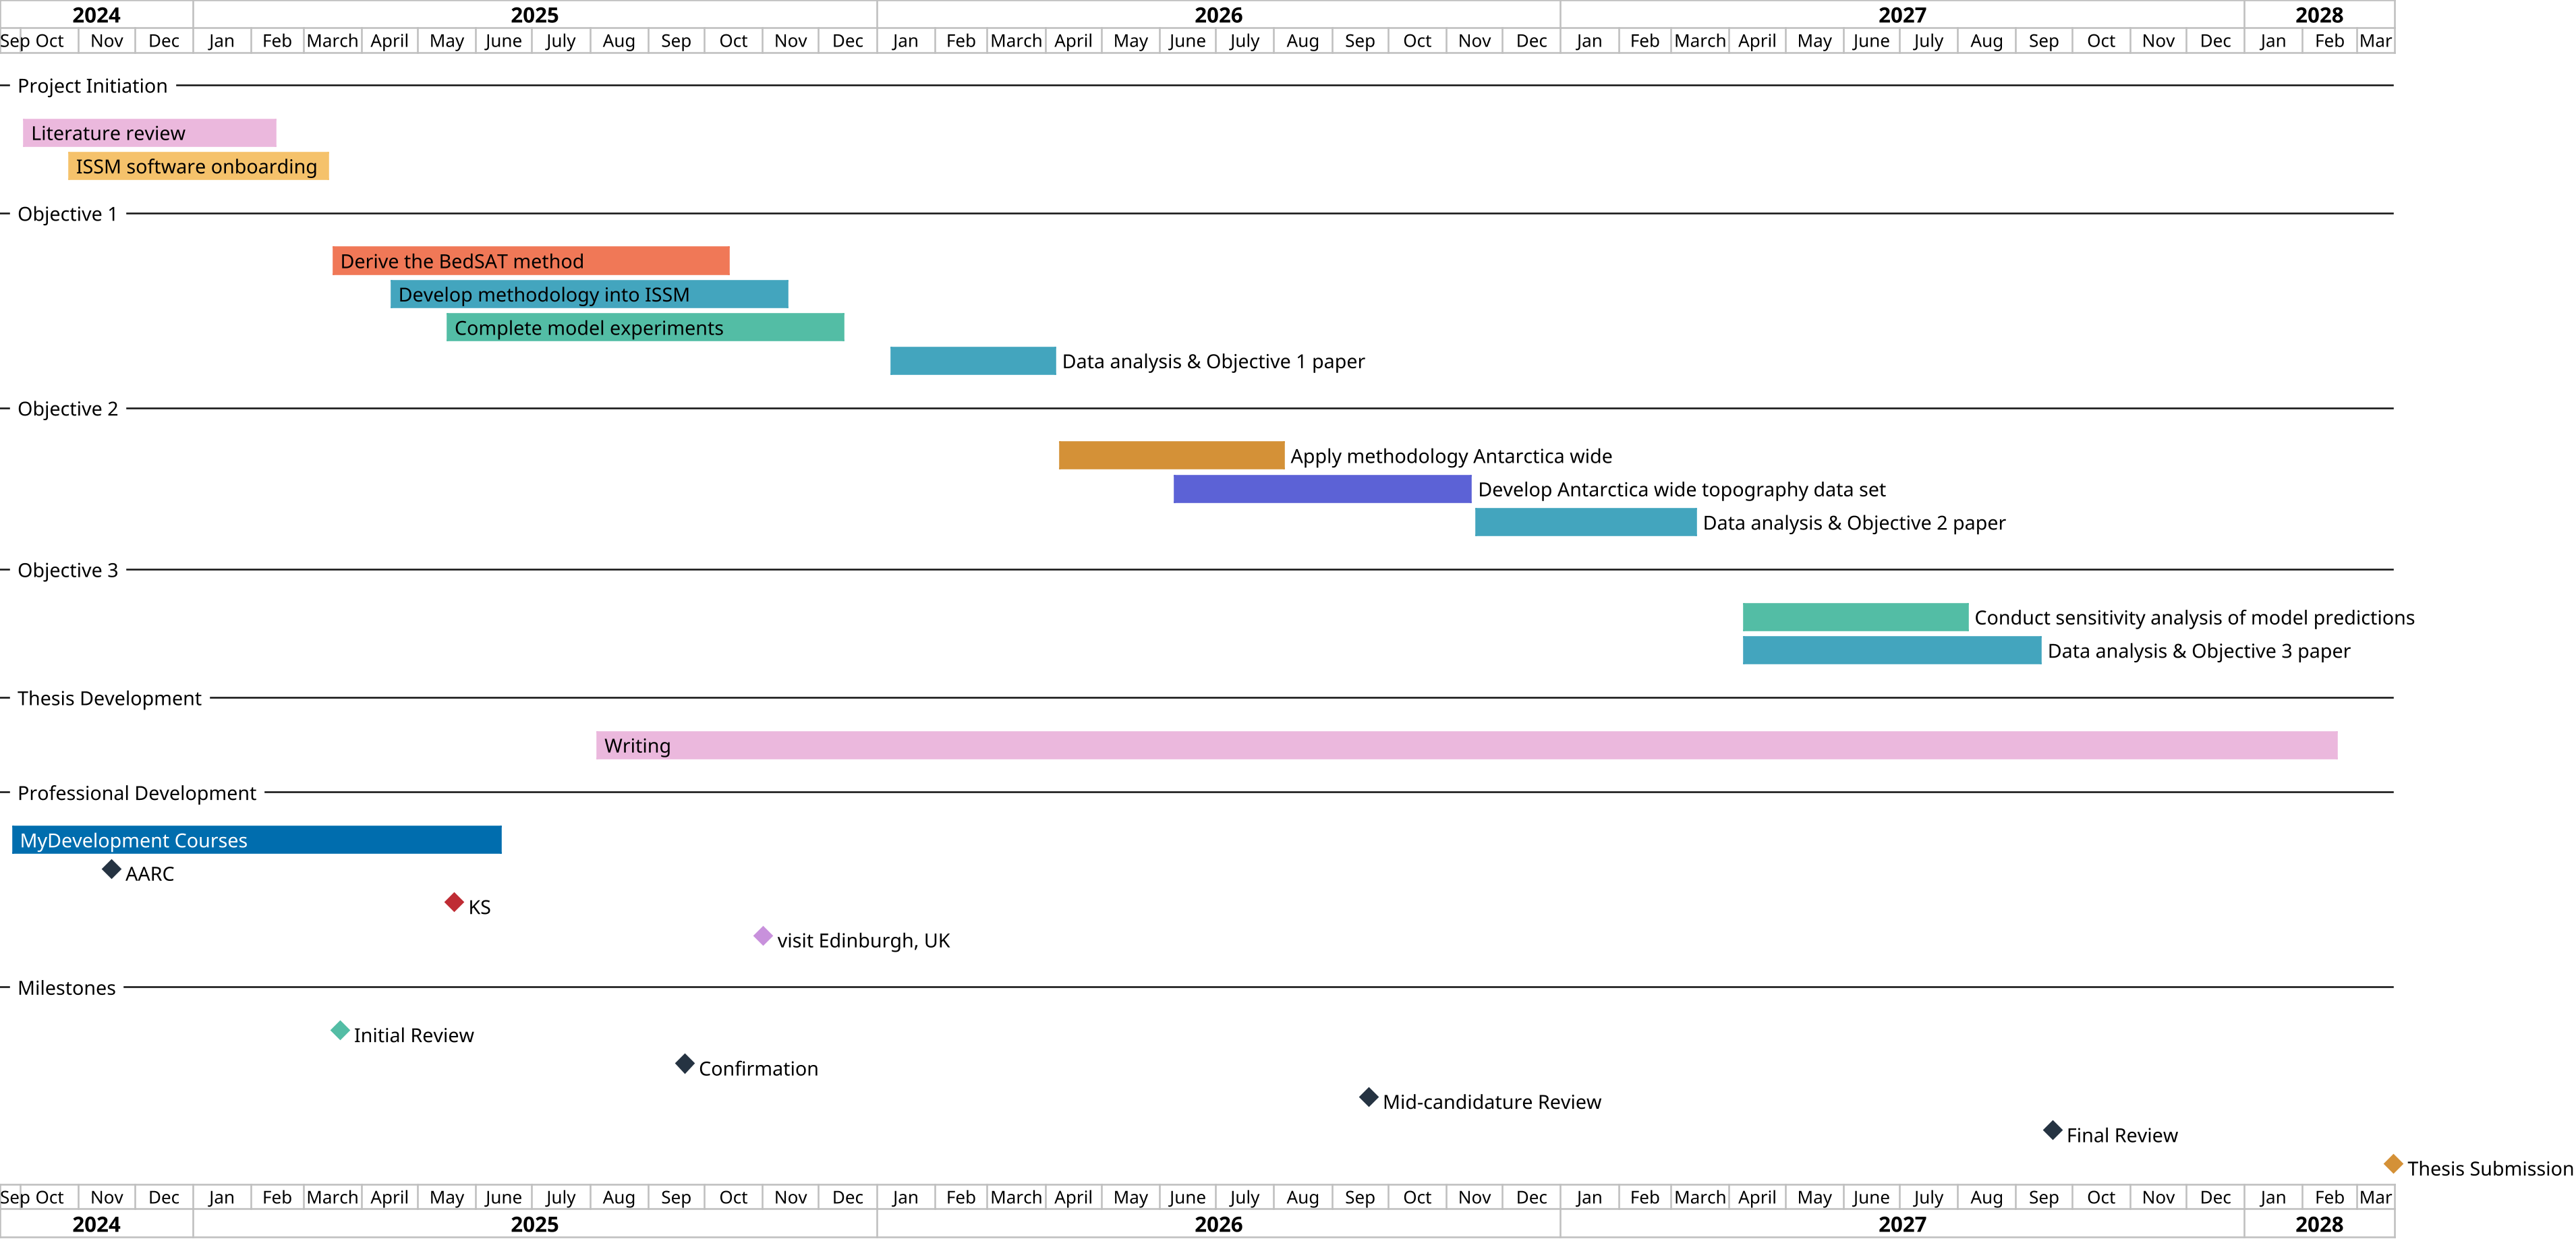
\includegraphics[width=\linewidth]{timeline.png}
\end{landscape}

\chapter{Glossary of Key Terms}\label{glossary}
\begin{enumerate}
\item \textbf{Adaptive Mesh Refinement}: A technique used to refine the mesh in regions of high variability or complexity, enhancing model accuracy and efficiency.
\item \textbf{Asperity}: A protrusion or bump on a surface. Roughness The unevenness of a surface, characterized by the size and distribution of asperities.
\item \textbf{Basal Drag Coefficient}: A parameter representing the frictional resistance between the ice sheet base and the underlying bedrock.
\item \textbf{Basal Melt Rates}: The rate at which the underside of a glacier or ice sheet melts due to contact with warmer ocean water.
\item \textbf{Basal sliding}: Sliding occurring at the base of a glacier.
\item \textbf{Bed Topography}: The shape and elevation of the bedrock underlying a glacier or ice sheet.
\item \textbf{Bedrock Topography}: The shape and elevation of the solid rock surface beneath a glacier or ice sheet.
\item \textbf{Blatter-Pattyn Approximation (BP)}: A higher-order ice flow model that incorporates longitudinal stresses, making it suitable for simulating fast-flowing ice streams and regions with significant vertical shear.
\item \textbf{Calving}: The process by which icebergs break off from the edge of a glacier or ice sheet.
\item \textbf{Coefficient of sliding friction ($\mu$)}: The ratio of the shear stress to the normal stress during steady-state sliding.
\item \textbf{Coefficient of static friction ($\mu_s$)}: The ratio of the limiting static shear stress to the normal stress, indicating the resistance to sliding from rest.
\item \textbf{Data Assimilation}: The process of incorporating observational data into a model to improve its accuracy and predictive capabilities.
\item \textbf{Finite Element Method (FEM)}: A numerical method for solving partial differential equations by dividing the domain into smaller elements and approximating the solution within each element.
\item \textbf{Fourier Transform}: A mathematical tool used to decompose a signal, such as surface elevation data, into its constituent frequencies. This allows for analysis of specific spatial scales and features.
\item \textbf{Full-Stokes (FS)}: The most comprehensive and computationally expensive ice flow model, accounting for all stress components. Essential for accurately simulating ice flow near grounding lines.
\item \textbf{Global Mean Sea-Level Rise (SLR)}: The average increase in sea level across the globe due to various factors, including melting of glaciers and ice sheets, and thermal expansion of ocean water.
\item \textbf{Grounding Line}: The boundary where the ice sheet transitions from grounded ice to floating ice (ice shelf).
\item \textbf{Ice-Penetrating Radar}: A remote sensing technique used to map the bedrock topography beneath glaciers and ice sheets by transmitting radar waves through the ice.
\item \textbf{Ice Sheet System Model (ISSM)}: A finite element, thermomechanical ice flow model that incorporates SIA, SSA, BP, and FS formulations to simulate ice sheet behaviour at various complexities and spatial resolutions.
\item \textbf{InSAR}: Interferometric Synthetic Aperture Radar, a remote sensing technique used to measure ice surface velocity.
\item \textbf{Inversion}: A mathematical technique used to infer unknown parameters, such as bed topography, from observations of other variables, such as surface elevation and velocity.
\item \textbf{Limiting dynamic shear stress ($T_m$)}: The shear stress at which a glacier or ice block transitions from steady-state sliding to accelerated sliding.
\item \textbf{Kriging}: A geostatistical interpolation method that estimates unknown values at specific points by calculating weighted averages of known values from surrounding points, while accounting for spatial correlation and providing uncertainty estimates.
\item \textbf{Limiting static shear stress ($T_S$)}: The minimum shear stress required to initiate sliding from a resting position.
\item \textbf{Linear Perturbation Analysis}: A technique that examines the response of a system to small perturbations in its parameters, assuming a linear relationship between the perturbation and the response.
\item \textbf{Marine Ice Sheet Instability (MISI)}: A process where the grounding line of an ice sheet retreats into deeper water, leading to accelerated ice discharge and potentially unstoppable collapse.
\item \textbf{Momentum Balance}: The fundamental physical principle describing how forces control ice motion, expressed through the Navier-Stokes equations. In ice sheet modeling, it accounts for the balance between internal stresses, gravitational driving forces, and resistive forces (including drag at the bed and lateral margins).
\item \textbf{Normal stress ($N$)}: The force acting perpendicular to a surface, per unit area. In the context of glaciers, it is primarily the weight of the overlying ice.
\item \textbf{Null Space}: The set of all possible solutions to an inverse problem that do not contribute to the observed data. In the case of the work of \ref{Ockenden_2022}, features aligned with ice flow fall within the null space and cannot be resolved by the inversion.
\item \textbf{Pinning Point}: A topographic feature, such as a ridge or mountain, that can slow or temporarily halt the retreat of a glacier's grounding line.
\item \textbf{Regelation}: The process of melting under pressure and refreezing at lower pressure, potentially contributing to ice sliding.
\item \textbf{Retrograde Bedrock Slope}: A bedrock slope that deepens inland, making the ice sheet more susceptible to marine ice sheet instability.
\item \textbf{Rheology}: The study of how materials deform and flow under stress. In glaciology, it refers to the flow properties of ice.
\item \textbf{Shallow Ice Approximation (SIA)}: A simplified ice flow model that considers only vertical shear stresses and neglects horizontal stress gradients. Suitable for slow-moving ice in the interior of ice sheets.
\item \textbf{Shallow Shelf Approximation (SSA)}: A simplified ice flow model that neglects vertical shear stresses and assumes depth-independent horizontal velocity. Appropriate for modelling floating ice shelves and fast-flowing ice streams.
\item \textbf{Shallow-Ice-Stream Approximation}: A simplification of the ice flow equations that assumes the ice thickness is much smaller than the horizontal extent of the glacier, allowing for analytical solutions.
\item \textbf{Shear stress ($T$)}: The force acting parallel to a surface, per unit area. In the context of glaciers, it is the force driving glacier motion.
\item \textbf{Sliding}: The movement of a glacier over its bed by sliding rather than internal deformation.
\item \textbf{Slipperiness}: A measure of the ease with which ice can slide over its bed. It encompasses the influence of basal conditions like geology, hydrology, and sediment characteristics.
\item \textbf{Steady-state}: A condition where the glacier's flow and properties are constant over time, assuming a balance between ice accumulation and loss.
\item \textbf{Steady-state velocity ($V_b$)}: The constant velocity reached by a glacier or ice block when the driving shear stress is balanced by resisting forces.
\item \textbf{Stress Balance}: The equilibrium between the forces acting on an ice sheet, including gravity, basal friction, and internal ice stresses.
\item \textbf{Temperate ice}: Ice at or near its pressure-melting point.
\item \textbf{Transfer Functions}: Mathematical equations that describe the relationship between perturbations in bed properties and the resulting changes in surface variables.
\item \textbf{Volume Above Floatation (VAF)}: The volume of an ice sheet that is grounded on bedrock and contributes to sea-level rise if it melts or slides into the ocean.
\item \textbf{Wavelet Decomposition}: A mathematical technique that analyzes a signal by decomposing it into different frequency components at various spatial scales.
\end{enumerate}
% \wordcount{glossary} words in this section.
% \include{dynamics}
% % \wordcount{dynamics} words in this section.
% %
% \include{Conclusion}
% % \wordcount{Conclusion} words in this section.
% %
% \appendix
% \include{appendix}
% % \wordcount{appendix} words in this section.

\bibliographystyle{unsrturl_mod}
\bibliography{mybib}
\end{document}


